The robot simulator V-REP, with integrated development environment, is based on a distributed control architecture: each object/model can be individually controlled via an embedded script, a plugin, a ROS node, a remote API client, or a custom solution. This makes V-REP very versatile and ideal for multi-robot applications. Controllers can be written in C/C++, Python, Java, Lua, Matlab, Octave or Urbi. \\

Previous to real implementation, in order to probe the effectiveness of the vision algorithm and the complete tracking architecture, the situation was simulated in this program. In this chapter will be described the process and the results of this simulations.

\subsection{The GUI}

In the following picture (Picture: \ref{fig:VREP_GUI}) shows the common user's interface of the simulator. At the top, there is the common edit buttons and camera movement through the scene. Also at the top on the right are the basic simulate configuration and buttons.

Some pre-created objects can be found in the model browser menu. There are a huge variety of mobile and fixed robots with their own AI and behavior integrated. This acts can be modified or amplified adding plugins or scripts as described previously.

Finally in the center of the interface the interface is the scene visualization. Objects are organized in the hierarchy menu on the left side of the scene.

\begin{figure}
	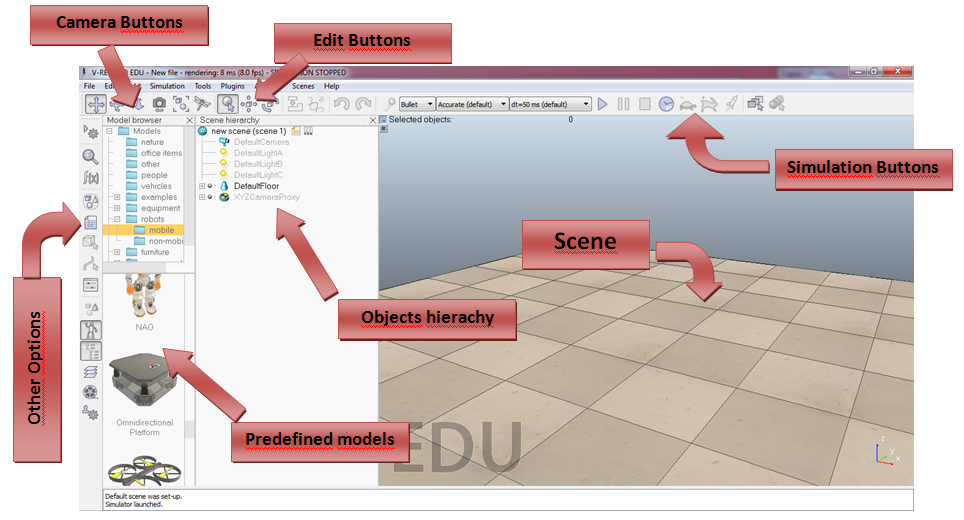
\includegraphics[width=\textwidth,natwidth=964,natheight=520]{../Images/c3/vrep_main.png}
	\caption{V-REP GUI}
	\label{fig:VREP_GUI}
\end{figure}


